%%%%%%%% ICML 2019 EXAMPLE LATEX SUBMISSION FILE %%%%%%%%%%%%%%%%%

\documentclass{article}

% Recommended, but optional, packages for figures and better typesetting:
\usepackage{microtype}
\usepackage{graphicx}
\usepackage{subfig}
\usepackage{booktabs} % for professional tables

% hyperref makes hyperlinks in the resulting PDF.
% If your build breaks (sometimes temporarily if a hyperlink spans a page)
% please comment out the following usepackage line and replace
% \usepackage{icml2019} with \usepackage[nohyperref]{icml2019} above.
\usepackage{hyperref}

% Attempt to make hyperref and algorithmic work together better:
\newcommand{\theHalgorithm}{\arabic{algorithm}}

% Use the following line for the initial blind version submitted for review:
\usepackage{icml2019}

% If accepted, instead use the following line for the camera-ready submission:
%\usepackage[accepted]{icml2019}

% The \icmltitle you define below is probably too long as a header.
% Therefore, a short form for the running title is supplied here:
\icmltitlerunning{System Identification through Expression Optimization}


%%%%%%%% this region contains all the stuff Anthony Added %%%%
\usepackage{bm}
\usepackage{amsfonts}
\usepackage{amsmath}
\newcommand{\todo}[1]{\textbf{[[#1]]}}
%%%%%%%%%%%%%%%%%%%%%%%%%%%%%%%%%%%%%%%%%%%%%%%%%%%%%%%%%%

\begin{document}

\twocolumn[
\icmltitle{System Identification through Expression Optimization}

% It is OKAY to include author information, even for blind
% submissions: the style file will automatically remove it for you
% unless you've provided the [accepted] option to the icml2019
% package.

% List of affiliations: The first argument should be a (short)
% identifier you will use later to specify author affiliations
% Academic affiliations should list Department, University, City, Region, Country
% Industry affiliations should list Company, City, Region, Country

% You can specify symbols, otherwise they are numbered in order.
% Ideally, you should not use this facility. Affiliations will be numbered
% in order of appearance and this is the preferred way.
\icmlsetsymbol{equal}{*}

\begin{icmlauthorlist}
\icmlauthor{Anthony Corso}{stanford}
\icmlauthor{Mykel Kochenderfer}{stanford}
\end{icmlauthorlist}

\icmlaffiliation{stanford}{Department of Aeronautics and Astronautics, Stanford University, Stanford, California, USA}

\icmlcorrespondingauthor{Anthony Corso}{acorso@stanford.edu}
\icmlcorrespondingauthor{Mykel Kochenderfer}{mykel@stanford.edu}

% You may provide any keywords that you
% find helpful for describing your paper; these are used to populate
% the "keywords" metadata in the PDF but will not be shown in the document
\icmlkeywords{Machine Learning, ICML}

\vskip 0.3in
]

% this must go after the closing bracket ] following \twocolumn[ ...

% This command actually creates the footnote in the first column
% listing the affiliations and the copyright notice.
% The command takes one argument, which is text to display at the start of the footnote.
% The \icmlEqualContribution command is standard text for equal contribution.
% Remove it (just {}) if you do not need this facility.

%\printAffiliationsAndNotice{}  % leave blank if no need to mention equal contribution
\printAffiliationsAndNotice{\icmlEqualContribution} % otherwise use the standard text.

\begin{abstract}
With the abundance of natural data from physical systems, much engineering and scientific value comes from an ability to discover the underlying, governing equations of a system, with little prior knowledge. Current approaches for data-driven system identification either find relationships in the data that aren't interpretable, or require significant prior knowledge from the user. This work describes a new approach to system identification that requires minimal user input and discovers governing equations that are parsimonious, generalizable and interpretable. This is enabled by recent advances in expression optimization, allowing for the automated discovery of mathematical expressions from a combinatorically large set of possibilities. Using simulated data, our approach correctly identifies both linear and nonlinear PDEs including the Navier-Stokes equations. It can also generate exact and approximate Koopman eigenfunctions for nonlinear ODEs. The ability to interpret large amounts of data will allow researchers to better understand and control important natural systems, such as the earth’s climate, for addressing global warming and fluid flow for more efficient energy generation and transportation.
\end{abstract}

\section{Introduction}
\label{introduction}

Over the past several decades machine learning and artificial intelligence has made great strides in learning patterns from large amounts of data. Although accurate, these systems are often uninterpretable by the human researchers who create them. They do not report an explanation for their predictions nor do they generalize well when the task is changed slightly.

Recently, however, strides have been made to create AI systems that, rather than just looking for trends, look for causal explanations of observed data (Bridewell, 2008, Brunton, 2016). If an AI system can correctly determine a simple underlying model for a system then it has the capability of providing an explanatory account of the data as well as the ability to generalize well in predicting behavior under a wider variety of situations. This can help researchers more quickly discover models that explain experimental data.

\todo{Describe the current systems and there limitations}

\todo{update the below paragraph to reflect the actual structure of the paper}
The goal of this project is to implement a system identifier for the discovery of physical processes in terms understandable by a human researcher (i.e. stated as partial differential equations (PDEs)). The system should work with multi-dimensional data, be robust to noise, and require small amounts of data to operate. This paper is outlined as follows: The next section discusses the approach to system identification that will be used, including how features are generated and selected from observed data. The following section describes two test systems from which synthetic noisy data is obtained to demonstrate the system identifier. The last two sections report the results of the system identifier and a discussion of how it can be improved.

\begin{itemize}
\item 
\item the drawback to other methods is that the user is responsible for defining which set of nonlinear functions should be used for the algorithm -- something that is not know a priori.
\item out approach is special because the use has to define only a context-fre grammar which can be very simple and yet lead to many complicated nonlinear features.
\item Grammars produce a combinatorically large number of possible expressions so we use an expression optimization technique to intelligently search the vast space of possibilites.
\end{itemize}


\section{System Identification}
\label{systemidentification}

The goal of identifying a simple model that describes observed data has been researched in the past by Bridewell, 2008, Brunton, 2016. The system identifier presented here, takes elements from those two approaches while expanding the capabilities to the domain of spatio-temporal processes governed by nonlinear PDEs. 

\subsection{Governing Equations}
The simplest form of a general PDE is given by
\[ \frac{\partial u(x,t)}{\partial t} = \alpha_1 f_1(u(x,t)) + ... + \alpha_n f_n(u(x,t)) = \bm{\alpha}^T \bm{f} \]
where the $\alpha_i$ are constant coefficients and the functions $f_i$ are \textit{feature functions} of the solution $u(x,t)$.

\todo{Describe the problem as a linear regression problem}
\todo{Transition using:}
we can think of the system identification task as finding a nonlinear mapping of the features that creates a linear relationship to the output data. If one were to look for a mapping, not just for the input data but for the output data as well, then you would be in the realm of koopman analysis.

\subsection{Koopman Eigenfunctions}
\todo{add importance of koopman solution} 

Koopman theory [CITATION] states that an nonlinear dynamical system can be converted into a linear system under the state space mapping
\[ \vec{x} \rightarrow \vec{g}(\vec{x}) \]
where $\vec{g}(x) = \begin{bmatrix} g_1(\vec{x}) & g_2(\vec{x}) & + & ... \end{bmatrix}$ and is, in general infinite dimensional.

Given the time-discrete nonlinear dynamical system given by
\[ \vec{x}^{t+1} = \vec{f}(\vec{x}^t)\]
the Koopman transformation yields the linear system
\[ \vec{g}(\vec{x})^{t+1} = K \vec{g}(\vec{x})^{t} \]

if the Koopman eigenfunctions contain the identity function $g(\vec{x}) = \vec{x}$ then the Koopman operator is said to be \emph{state-inclusive} and the untransformed state of the system can be found directly from the linear system, without finding an inverse transformation $\vec{g}^{-1}$.


\subsection{Past Approaches}
\begin{itemize}
    \item Sindy and Langley's work where you have to specify entire features
    \item DMD where you get a low dimensional approximation without much user input but the resulting modes don't make contact with domain specific content.
\end{itemize}


\todo{add a transition to the next paragraph where we discuss a new design approach based on expression optimization which alleviates some of these issues}

The first step of the system will be to generate a large number of feasible feature functions that could comprise the PDE. The second step is to select a subset of these features that best explain the left hand side of the PDE through linear regression. These steps are discussed in more detail in the next few subsections.

\section{System Identification through Expression Optimization (SIEO)}
\begin{itemize}
    \item Define a grammar (Context-Free Grammars)
    \item Define an objective function (subsection: Objective Function)
    \item select the subset of features from the grammar that best describe the data based (Search algs -- which combine expression optimization, forward search and backward search)
\end{itemize}

\subsection{Context-Free Grammar}

The choice of feature selection in general is a difficult problem. There are an infinite number of possible feature functions and it is impossible to know a priori which functions will comprise the PDE. Since the system identifier is meant to be an aide to researchers and scientists, it is reasonable to ask the user to provide some amount of guidance to the algorithm without explicitly handing over a set of feature functions (which the researcher presumably does not know).

To this end, the system identifier relies on a domain-specific \textit{grammar}, provided by the user, that gives the rules for generating feature functions. A grammar is a set of production rules that govern a language (or a set of expressions). Each rule can either be \textit{non-terminal}, in which the rule relates generic expressions together (e.g. multiplication), or \textit{terminal}, in which an expression is concretely defined (e.g. the observed data). Each expression in the language can be represented by a tree of operators, each of which is part of the grammar. Once a grammar is defined, expressions can be sampled from the grammar with varying levels of complexity (as defined by the depth of the expression tree).

A sample grammar and expression tree are shown in figure \ref{fig:grammar}. A convenient way to read the rules of the grammar is to convert it to plain english. Let $\mathbb{R}$ mean ``an expression'' and $\mapsto$ mean ``can be'', then the second production rule reads ``an expression can be an expression times an expression''. The last production rule is where the variables of interest are introduced. This rule reads ``an expression can be a velocity component or pressure''. Sampling from a grammar is a process of selecting production rules and then filling in any non-terminal expressions until only terminal expressions remain. In the expression tree shown in the right of figure \ref{fig:grammar}, the first production rule chosen is multiplication. Then, on the left side, the terminal expression $u$ was chosen, and on the right side, the spatial derivative was chosen, followed by the terminal expression $u$.

To produce the candidate set of features, the user will specify a desired tree depth, $d$, and all possible expressions with depth $\leq d$ will be produced. Then, this set of features is searched for expressions that evaluate to the same results and any such duplicates are removed. The number of candidate expressions grows exponentially with the depth of the tree, but fortunately, most pdes that govern physical processes have terms that are only at a depth of 4 or less which makes the problem tractable (see Wikipedia list of nonlinear PDEs, 2018). For the model systems, all terms can be produced from an expression depth of 3, which, for the grammar in figure \ref{fig:grammar} means that a total of 562 features will be considered (222 after removing duplicates). The julia package \verb|ExprRules.jl| was used to build the grammar and to sample expressions from it at the desired depth.

\subsection{Choice of Objective Function}

The metric that was chosen to decide between models is the adjusted $R^2$ value of the fit. The traditional $R^2$ value always increases when new features are added so it makes our algorithm susceptible to overfitting. Instead, we penalized the addition of more features to the regression by defining the $R_{\rm adj}^2$ as [CITATION]
\[ l_f = -R_{\rm adj}^2 = -[R^2 - \alpha (1-  R^2)(n-1)]\]
where $n$ is the number of features in the model.

Note that when $n=1$, this expression reduces to the traditional $R^2$ value. But when $n>1$, then the difference between $R^2$ and 1 is scaled by the number of parameters. Thus, as a rule of thumb, $\alpha \in [0, \infty)$ should be large when you expect there to be excellent agreement between the input and output (i.e. for synthetic, noise-free data) and should be closer to 0 when near-perfect agreement is not expected (i.e. real world data).

In the case of discovering Koopman modes, parsimony is no longer a consideration so a new objective function needs to be used. Given a linear system with $n_g$ number of Koopman eigenfunctions, the loss function associated with the Koopman operator $K$ and Koopman eigenfunction $\vec{g}$ is given by

\[ l_k(K, \vec{g}) = \frac{1}{n_g}||\vec{g}(\vec{x})^{t+1} - K \vec{g}(\vec{x})^{t}||_2^2 \]

The scaling by $1/n_g$ is so that that algorithm does not get penalized for adding more Koopman eigenfunctions to explain the system, and instead focuses on closely matching each new state variable on each iteration.


\subsection{Feature Selection Algorithms}

\todo{outline the high level approach to the system}

\subsubsection{Feature Selection}
The problem selecting amongst a group of possible features is a challenging one. If there are $N$ possible features then there are $2^N$ possible subsets to choose. It is infeasible to search the entire space of combinations so certain heuristics need to be employed. 

Previous approaches have used sparsity-promoting regression techniques such as LASSO [Citation] but these can pose difficulties when the features suffer from mulicollinearity [ PDE citation]. In this work, the heuristic that performed the best was a modified form a greedy feature selection algorithm that combined both forward and backward search. The high-level structure of the algorithm is given in Algorithm \ref{alg:featureselection}.

The algorithm starts by performing a greedy forward search (Algorithm \ref{alg:forwardsearch}), where, on each iteration, the feature that leads to the largest decrease in the cost function is added to the expression until there is no further improvement or a specified threshold is hit. Then, the feature selection algorithm performs a greedy backward search on the expression (Algorithm \ref{alg:backwardsearch}), where features are removed if their absence reduces the cost function. This entire process iterates until there is no further improvement of the expression, at which point this individual is returned.

\begin{algorithm}[tb]
   \caption{Feature Selection}
   \label{alg:featureselection}
\begin{algorithmic}
   \STATE {\bfseries Input:} Loss function $l_f$, \\
   \quad \quad \quad New feature generator $n_f$, \\
   \quad \quad \quad Threshold $t$ \\
   \STATE Initialize $expr = [ \ ]$
   \REPEAT
   \STATE $old_expr = expr$
   \STATE $expr = {\rm forward_search}(expr, lf, n_f, t)$
   \STATE $expr = {\rm backward_search}(expr, lf, n_f, t)$
   \UNTIL $old_expr == expr$
\end{algorithmic}
\end{algorithm}

\begin{algorithm}[tb]
   \caption{Forward Search}
   \label{alg:forwardsearch}
\begin{algorithmic}
   \STATE {\bfseries Input:} Loss function $l_f$, \\
   \quad \quad \quad Expression $expr$, \\
   \quad \quad \quad New feature generator $n_f$, \\
   \quad \quad \quad Threshold $t$ \\
   \STATE Initialize $lowest = l_f(expr)$
   \REPEAT
   \STATE $expr = {\rm concatenate}(expr, \ n_f(expression))$
   \IF{$l_f(expr) < lowest$}
   \STATE $lowest = l_f(expr)$
   \ELSE
   \STATE {\bfseries return} $expr$
   \ENDIF
   \UNTIL $lowest < t$
\end{algorithmic}
\end{algorithm}

\begin{algorithm}[tb]
   \caption{Backward Search}
   \label{alg:backwardsearch}
\begin{algorithmic}
   \STATE {\bfseries Input:} Loss function $l_f$, \\
   \quad \quad \quad Expression $expr$, \\
   \quad \quad \quad Threshold $t$ \\
   \STATE Initialize $lowest = l_f(expr)$
   \REPEAT
   \STATE Initialize $losses = [ \ ]$
   \FOR{$feat$ {\bfseries in} $expr$}
   \STATE $new_expr = {\rm remove}(expr, feat)$
   \STATE ${\rm push}(losses, l_f(new_expr))$
   \ENDFOR
   \STATE $i = {\rm arg\,max}(losses)$
   \IF{$losses[i] < lowest$}
   \STATE $lowest = losses[i]$
   \STATE $expr = {\rm remove}(expr, feat)$
   \ELSE
   \STATE {\bfseries return} $expr$
   \ENDIF
   \UNTIL $lowest < t$
\end{algorithmic}
\end{algorithm}


\subsubsection{Expression Optimization}
\todo{topic paragraph on the generation of new features and why that is challenging}
\todo{transition to using Expression optimization techniques and specifically grammatical evolution}

Grammatical Evolution is an expression optimization approach introduced by [CITATION]. Each feature that is sampled from the grammar is expressed as an unbounded integer array that can be parsed from left to right into an expression tree. Each integer array is transformed in a manner similar to genetic algorithms. The basic operations are
\begin{enumerate}
\item \textbf{Selection} - The integer arrays with the best fitness (lowest cost function) are selected from the population
\item \textbf{Crossover} - The fittest individuals produce offspring that carry traits from the parents
\item \textbf{Mutation} - The integer arrays are randomly altered (while preserving the rules of the grammar)
\item \textbf{Gene Duplication} - Where useful genes are copied in the integer array so that they are less likely to be lost
\item \textbf{Pruning} - Some integer arrays will contain genetic information that is unused (put there through crossover). So with some probability unused genes are pruned in an individual.
\item
\end{enumerate}

These operations are applied to a large number of individuals over many generations in order to produce optimal features from the large space of possibilities.


\section{Results}
\label{results}
SIEO was tested on four separate model problems to demonstrate its capabilities and probe its robustness. The first two problems are PDES. The first is used to demonstrate the algorithms robustness to noise and limited spatial sample points. The second is to demonstrate that the algorithm scales to problems with multiple spatial dimensions and multiple variables. The next two test cases show the utility of SIEO for approximating Koopman functions, first finding them exactly and then finding good approximation.

\subsection{Advection-Diffusion Equation}

The first model problem is the unsteady 1D advection-diffusion equation which describes the general linear transport of material $u$ in a fluid. The governing equation has the form 
\begin{equation} 
\frac{\partial u}{\partial t} = D\frac{\partial^2 u}{\partial x^2} - v \frac{\partial u}{\partial x}
\end{equation}
where $D$ is the diffusion coefficient, $v$ is the fluid velocity. Synthetic data is generated using the exact solution derived by (Van Genuchten 1982) which for boundary conditions 
\begin{align}
  u(x,0) &= u_0 \\
  u(0,t) &= u_L \\
  \frac{\partial u}{\partial x}(\infty, t) &= 0
\end{align}
is found to be 
\begin{equation}
  \begin{split}
  u(x,t) = u_0 + \frac{1}{2}&(u_L - u_0) \left({\rm erfc}\left[ \frac{x - vt}{2\sqrt{Dt}}\right]\right. \\
  &+ \left.{\rm exp}(vx/D) {\rm erfc}\left[ \frac{x + vt}{2\sqrt{Dt}}\right] \right)
  \end{split}
\end{equation}
This solution is plotted in figure \ref{fig:advdif} for $x>0$, $t>0$, $D=1$, $v=1$, and $U_L = 1$.

\begin{figure}
\vskip 0.2in
\begin{center}
\centerline{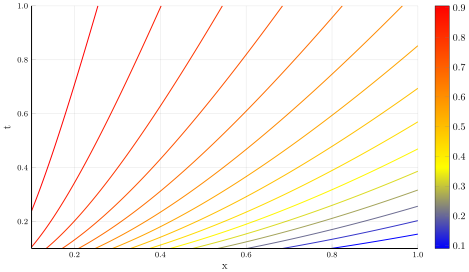
\includegraphics[width=\columnwidth]{./figures/advdif}}
\caption{Unsteady data from the 1D advection-diffusion equation}
\label{fig:advdif}
\end{center}
\vskip -0.2in
\end{figure}

To apply SIEO the exact solution was sampled at 200 temporal points in the range $t = (0, 0.1)$ and between 10 and 200 spatial points . Then, additive white Gaussian noise at a level $\eta \in (0, 0.2)$ was added to the data such that the standard deviation of the noise is given by $\sigma = \eta \ {\rm std}(u)$. The grammar shown in figure \ref{fig:advdifgrammar} was used for the expression optimization routine and was limited to a tree depth of 3. The adjusted $R^2$ loss function was used with the parameter $\alpha = 0.5$. The solution was denoised using total variation filtering [tv citation] both before and after the numerical differentiation.
\begin{figure}
    \vskip -0.2in
    \centering
    \begin{equation*}
    \begin{split}
    \mathbb{R} &\mapsto u \\
    \mathbb{R} &\mapsto \frac{d\mathbb{R}}{dx} \\
    \mathbb{R} &\mapsto \mathbb{R} \times \mathbb{R} \\
    \mathbb{R} &\mapsto \mathbb{R} / \mathbb{R}
    \end{split}
    \end{equation*}
    \vskip -0.15in
    \caption{Grammar used for the advection-diffusion equation}
    \label{fig:advdifgrammar}
    \vskip -.15in
\end{figure}
The results of six testcases are shown in table \ref{tab:advdifresults}. After the trial number, the first two columns show the number of spatial sample points used and the noise level, respectively. The last two columns show the percent error in the model parameters, $v$ and $D$ when compared to their exact values. In all six testcases, SIEO determined the correct form of the governing equation. When the noise is 1-5 \% and the number of sample points is 35 or larger, the error in the parameters remains small. In the two most challenging testcases (trials 3 and 6), the fit parameters $v$ and $D$ show high levels of error but the correct form the equation was still discovered accurately which demonstrates the robustness of SIEO to find an accurate and generalizable model with large amounts of noise or limited data.

\begin{table}[t]
\caption{Error in solution parameters for different noise levels and spatial resolutions}
\label{tab:advdifresults}
\vskip 0.15in
\begin{center}
\begin{small}
\begin{sc}
\begin{tabular}{lccccr}
\toprule
 & Sample &  & Error & Error\\
Trial & Points & Noise & in $v$ & in $D$\\
\midrule
1 & 200 & 1\%  & 0.78 \% & 1.54 \% \\
2 & 200 & 5\%  & 5.64 \% & 2.84 \% \\
3 & 200 & 20\%  & 30.12 \% & 6.60 \% \\
4 & 100 & 0\%  & 0.84 \% & 0.29 \% \\
5 & 35 & 0\%  & 6.38 \% & 2.21 \% \\
6 & 10 & 0\%  & 1.19 \% & 19.02 \% \\
\bottomrule
\end{tabular}
\end{sc}
\end{small}
\end{center}
\vskip -0.1in
\end{table}


\subsection{Navier-Stokes Equations}
The second test system is the incompressible 2D Navier-Stokes equations which describe the motion of a viscous fluid. The Navier-Stokes equations are given by
\begin{align}
  \frac{\partial u}{\partial x} + \partial{v}{\partial y} &= 0 \\
  \frac{\partial u }{\partial t} + u \frac{\partial u }{\partial x} + v \frac{\partial u }{\partial y} &= - \frac{1}{\rho} \frac{\partial p}{\partial x} + \frac{\mu}{\rho}\left( \frac{\partial^2 u}{\partial x^2} + \frac{\partial^2 u}{\partial y^2} \right) \\
\frac{\partial v }{\partial t} + u \frac{\partial v }{\partial x} + v \frac{\partial v }{\partial y} &= - \frac{1}{\rho} \frac{\partial p}{\partial v} + \frac{\mu}{\rho}\left( \frac{\partial^2 v}{\partial x^2} + \frac{\partial^2 v}{\partial y^2} \right)
\end{align}

where $\rho$ is the fluid density, $(u, v)$ is the fluid velocity, $p$ is the pressure, and $\mu$ is the viscosity. The first equation represents the conservation of mass and the next two equations represent conservation of momentum in the $x$ and $y$ directions, respectively. These equations are nonlinear, have multiple dimensions ($x$ and $y$) and multiple degrees of freedom ($u$, $v$, and $p$), which makes them a challenging test case for system identification.

Synthetic data was collected from the simulation of vortex shedding behind a circular cylinder at a Reynold's number of 50. The simulation was performed using \emph{PyFR} [citation] and 10 snapshots were taken with a timestep of $dt = 0.001$, $M = 0.2$ and $\rho \approx 1$ (with a very small amount of compressibility in the solution). A single frame of the simulation is shown in figure \ref{fig:ns_data}, with $u$, $v$, and $p$ on separate plots. The grammar in figure \ref{fig:nsgrammar} was used to produce features up to a depth of 3, yielding 363 features and $2^{363}$ expressions to be searched.

\begin{figure}
  \vskip 0.2in
    \subfloat[$x$-velocity]{\label{xvelocity}\includegraphics[width=\columnwidth]{./figures/xvel}} \\
    \subfloat[$y$-velocity]{\label{yvelocity}\includegraphics[width=\columnwidth]{./figures/yvel}} \\
    \subfloat[pressure]{\label{pressure}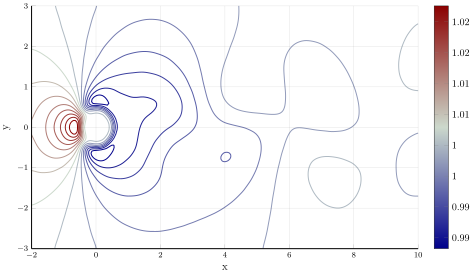
\includegraphics[width=\columnwidth]{./figures/pressure}}
    \caption{Global caption that can reference \ref{sublable1} and \ref{sublable2}}
    \label{fig:ns_data}
    \vskip -0.2in
\end{figure}

\begin{figure}
\vskip -0.15in
\centering
    \begin{equation*}
        \begin{split}
          \mathbb{R} &\mapsto u \quad | \quad v \quad | \quad p \\
          \mathbb{R} &\mapsto \frac{d\mathbb{R}}{dx} \quad \left| \quad \frac{d\mathbb{R}}{dy} \right. \\
          \mathbb{R} &\mapsto \mathbb{R} \times \mathbb{R}
        \end{split}
    \end{equation*}
    \vskip -0.15in
    \caption{Grammar used for the Navier-Stokes equations}
    \label{fig:nsgrammar}
    \vskip -.15in
\end{figure}

SIEO was performed on the the vortex shedding data with the adjusted $R^2$ loss function and $\alpha = 0.2 $. The algorithm found equations \ref{eqn:xmom} and \ref{eqn:ymom} to explain the unsteady Navier-Stokes data
\begin{align}
\label{eqn:xmom}
    \frac{\partial u}{\partial t} &= {\theta_x}_1 \frac{\partial}{\partial y} (u v) + {\theta_x}_2 v \frac{\partial u}{\partial y} + {\theta_x}_3 \frac{\partial p}{\partial y} + {\theta_x}_4 \frac{\partial^2 u}{\partial y^2} \\
\label{eqn:ymom}
    \frac{\partial v}{\partial t} &= {\theta_y}_1 u \frac{\partial v}{\partial x} (u v) + {\theta_y}_2 v \frac{\partial v}{\partial y} + {\theta_y}_3 \frac{\partial p}{\partial y}
\end{align}
Note that the first equation requires the substitution $\partial v /\partial y = - \partial u / \partial x $ (from the continuity equation) to transform it to the more well-known form of the $x$-momentum equation. Also note the absence of the viscous terms $\partial^2 u / \partial x^2$, $\partial^2 v / \partial x^2$, and $\partial^2 v / \partial y^2$. These terms are not included because in this particular fluid flow they are much smaller in magnitude than the other terms in the governing equation. This shows that for SIEO to identify a process, that process must be sufficiently active in the data collected. 

The ratios of the model coefficients were compared to get a sense of the error in the model parameters. The results are shown in table \ref{tab:ns_data}. In general, the model parameter error is very small and the discovered equations could be used for prediction or control of other similar types of flow field (i.e. those that don't have significant contributions from the viscous terms).

\begin{table}[t]
\caption{Error in Navier-Stokes Coefficients}
\label{tab:ns_data}
\vskip 0.15in
\begin{center}
\begin{small}
\begin{sc}
\begin{tabular}{lccccr}
\toprule
Parameter & Error \\
\midrule
${\theta_x}_2 / {\theta_x}_1 $ & 2.87 \% \\
${\theta_x}_3 / {\theta_x}_1 $ & 1.00 \% \\
${\theta_x}_4 / {\theta_x}_1 $ & 2.53 \% \\
${\theta_y}_2 / {\theta_x}_1 $ & 8.47 \% \\
${\theta_y}_3 / {\theta_x}_1 $ & 0.92 \% \\
\bottomrule
\end{tabular}
\end{sc}
\end{small}
\end{center}
\vskip -0.1in
\end{table}

\subsection{Exact Koopman Eigenfunction Discovery}
\label{exactdiscovery}
A simple nonlinear ODE with an easily found, and finite-dimensional Koopman eigenfunctions is given by [Brunton citation]
\begin{equation}
\begin{split}
  \label{simplekoopman}
\frac{dx}{dt} = \mu x \\
\frac{dy}{dt} = \lambda(y - x^2)
\end{split}
\end{equation}
The state-space transformation
\begin{equation}
    \label{eqn:exacttransform}
\begin{bmatrix}
x\\
y
\end{bmatrix} \Rightarrow \begin{bmatrix}
x \\
y \\
x^2
\end{bmatrix}
\end{equation}
linearizes equation \ref{simplekoopman} to
\begin{equation}
    \label{eqn:koopmanop}
\frac{d}{dt} \begin{bmatrix}
x \\
y \\
x^2
\end{bmatrix} = \begin{bmatrix}
\mu & 0 & 0 \\
0 & \lambda & -\lambda \\
0 & 0 & 2 \mu
\end{bmatrix} \begin{bmatrix}
x \\
y \\
x^2
\end{bmatrix}
\end{equation}

To test the discovery of exact Koopman operators, data from the system (\ref{simplekoopman}) was collected data for many initial conditions. The initial data is stored in a vector $\vec{x}^0$, then the solution is integrated forward one timestep and the result is stored in another vector $\vec{x}^1$. SIEO was then applied with the average sum of squares loss function $l_k$. The goal was to find a state-inclusive Koopman operator so the loss function was modified to penalize the absence of the primary state variables $x$ and $y$. The function-rich grammar in figure \ref{fig:odegrammar} was used as input (exchanging ($\theta$, $\omega$) for ($x$, $y$)). The correct Koopman transformation was discovered (equation \ref{eqn:exacttransform}) and the Koopman operator (equation \ref{eqn:koopmanop}) was recovered to within machine precision.







\subsection{Approximate Koopman Eigenfunction Discovery of Nonlinear Pendulum}
One of the simplest nonlinear ODEs without a known Koopman operator, is a simple pendulum swinging at large angles. The equation of motion a pendulum is given by
\[ \frac{d^2 \theta}{d t^2} + \sin \theta = 0 \]
This equation can be converted to a system of nonlinear first-order ODEs given by
\begin{align*}
\frac{d\theta}{dt} &= \omega \\
\frac{d\omega}{dt} &= -\sin \theta
\end{align*}


\begin{figure}
\vskip -0.15in
\centering
\begin{equation*}
    \begin{split}
        \mathbb{R} &\mapsto \theta \quad | \quad \omega \\
        \mathbb{R} &\mapsto \mathbb{R} \times \mathbb{R} \\
        \mathbb{R} &\mapsto \sin (\mathbb{G} \times \mathbb{R}) \quad | \quad \sin (\mathbb{G} \times \mathbb{R} + \mathbb{G}) \\
        \mathbb{R} &\mapsto {\rm exp}(\mathbb{G} \times \mathbb{R}) \\
        \mathbb{R} &\mapsto 1 / (1 + {\rm exp}(-\mathbb{G} \times \mathbb{R})) \\
        \mathbb{R} &\mapsto {\rm exp}(-(\mathbb{R}-\mathbb{G})^2/\mathbb{G}) \\
        \mathbb{R} &\mapsto {\rm imag}(\mathbb{R}^\mathbb{G}) \\
        \mathbb{R} &\mapsto {\rm real}(\mathbb{R}^\mathbb{G}) \\
        \mathbb{G} &\mapsto -\mathbb{G} \quad | \quad \mathbb{G}+\mathbb{G} \quad | \quad \mathbb{G}/\mathbb{G} \\
        \mathbb{G} &\mapsto {\rm logspace(-5, 2, 20)}
    \end{split}
\end{equation*}
    \vskip -0.15in
    \caption{Grammar used for both nonlinear ODEs}
    \label{fig:odegrammar}
    \vskip -.15in
\end{figure}


\todo{section on methods}
In order to generate training data, the system was integrated forward in time from a starting position $(\theta_0, \omega_0) = (\pi/2, 0)$ until $T=10$. Koopman operator was approximated by SIEO using the average sum of squares loss function with the same state-inclusive penalty described in section \ref{exactdiscovery}. The function-rich grammar shown in figure \ref{fig:odegrammar} was used as the input. The resulting expression with $24$ features was then compared to a linearized version of the equation with only the primary state variables. Both linear models were initialized at $(\theta_0, \omega_0) = (\pi/2, 0)$ and were allowed to evolve forward in time past the training period. The error between the linear model and the exact solution for each model is shown in figure \ref{fig:pendulum}.

The figure shows that the linear model with more nonlinear features has significantly lower average error then the linear model with only the two state variables. Additionally, the error more slowly for the Koopman approximation. This shows that it is possible to improve linearizations of nonlinear model by using expression optimization to approximate the Koopman eigenfunctions of the system.

\begin{figure}
\vskip 0.2in
\begin{center}
\centerline{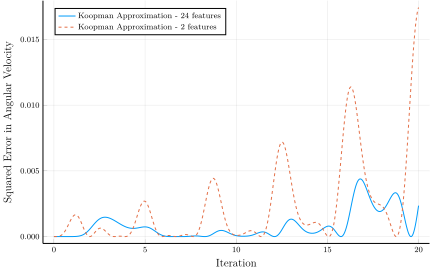
\includegraphics[width=\columnwidth]{./figures/pendulum}}
\caption{Error in the nonlinear pendulum for the simplest linear model and linear model with more nonlinear features}
\label{fig:pendulum}
\end{center}
\vskip -0.2in
\end{figure}

\section{Conclusions}

\begin{itemize}
    \item robustness in equation form to noise limited data and suggests that these types of models will be more generalizabile and reusable than a model that is opaque. this is because we are still able to glean relationships from the data without explaining it exactly.
\end{itemize}

\todo{Summarize and conclude}



% Acknowledgements should only appear in the accepted version.
% \section*{Acknowledgements}

% In the unusual situation where you want a paper to appear in the
% references without citing it in the main text, use \nocite
\nocite{langley00}

\bibliography{example_paper}
\bibliographystyle{icml2019}


\end{document}


% This document was modified from the file originally made available by
% Pat Langley and Andrea Danyluk for ICML-2K. This version was created
% by Iain Murray in 2018, and modified by Alexandre Bouchard in
% 2019. Previous contributors include Dan Roy, Lise Getoor and Tobias
% Scheffer, which was slightly modified from the 2010 version by
% Thorsten Joachims & Johannes Fuernkranz, slightly modified from the
% 2009 version by Kiri Wagstaff and Sam Roweis's 2008 version, which is
% slightly modified from Prasad Tadepalli's 2007 version which is a
% lightly changed version of the previous year's version by Andrew
% Moore, which was in turn edited from those of Kristian Kersting and
% Codrina Lauth. Alex Smola contributed to the algorithmic style files.
